\section{Módulo de Decodificação}
\label{sec:modulo_decodificacao}

	Conhecendo a imagem do marcador encontrado cabe a este módulo extrair a informação representada por 
	ele. Para isto são utilizados marcadores QRCode ao qual representa o nome do dispositivo. Desta forma é 
	possível encontrar os recursos (\textit{drivers}) por este disponibilizados. Assim como o Módulo de Reconhecimento, 
	este módulo consiste em uma linha de execução própria e seu fluxo de execução ocorre conforme representado 
	na Figura \ref{fig:processo_decode} e descrito a seguir.
	
	\begin{figure}[htb]
		\centering 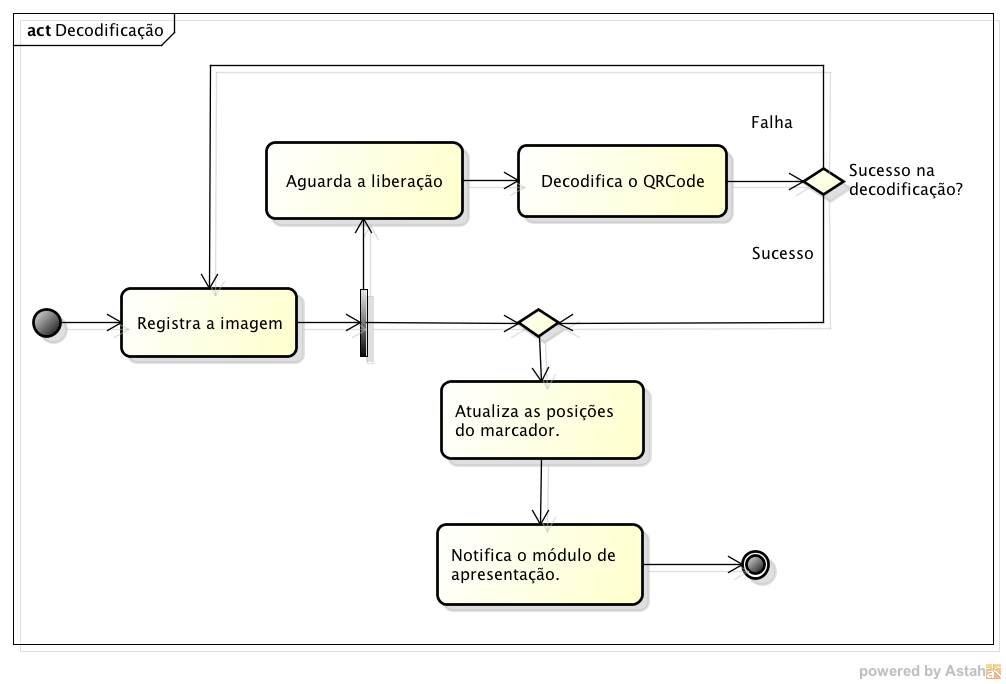
\includegraphics[scale=0.6]{figuras/cap4/processo_decodificacao.png}
		\caption{\textit{Processos do Módulo de Decodificação.}}
		\label{fig:processo_decode} 
	\end{figure}
	
	O Módulo de Decodificação é criado junto com o módulo de Reconhecimento, no entanto sua execução é 
	iniciada após o recebimento de algum marcador encontrado pelo Módulo de Reconhecimento. O marcador 
	recebido é registrado para que seja feito a atualização das informações a respeito da imagem recebida.
	Com o registro efetuado com sucesso é dado início ao processo de decodificação do marcador recebido. 
	Pelo fato do processo de reconhecimento ser mais rápido quando comparado ao processo de decodificação
	fez-se necessário a criação de um controle para que fosse garantido uma correta sincronização na 
	decodificação dos marcadores. Por essa razão, ocorrerá o descarte de qualquer marcador recebido enquanto 
	houver um processo de decodificação em execução. 
	
	Foi criado um Gerenciador com o propósito de centralizar todas as informações necessárias, de classes e 
	procedimentos, envolvidas no processo de decodificação. Ele age como uma interface entre o Módulo de 
	Decodificação e as aplicações responsáveis pela decodificação. A aplicação ZBar~\cite{zbar} foi utilizada 
	como ferramenta suporte ao processo de decodificação. Esta ferramenta é implementada utilizando a linguagem C. 
	Por essa razão a integração entre a aplicação ZBar com a ARHydra ocorre através do JNI. 
	
	As posições do marcador são atualizadas após o processo de decodificação ser finalizado com sucesso, ou seja, 
	houve êxito na obtenção do código de identificação do marcador analisado. Essa mesma etapa correspondente a  
	atualização das posições é feita quando um marcador é recebido do Módulo de Reconhecimento. Essa tarefa tem 
	um comportamento assíncrono devido o processo de decodificação ser um processo oneroso quando comparado dos 
	demais procedimentos separadamente. Por essa razão, enquanto houver um processo de decodificação em execução, as 
	posições referentes ao objeto virtual apresentado ao usuário são atualizadas com as informações recebidas
	pelos marcadores enviadas do Módulo de Reconhecimento. Após a atualização, essas informações são repassadas 
	ao Módulo de Apresentação para que as informações correspondentes ao marcador sejam atualizadas e apresentadas 
	ao usuário.
	
	Por outro lado, caso o processo de decodificação não consiga obter o código identificador correspondente ao 
	marcador analisado, o Módulo de Decodificação enviará uma notificação para o Módulo de Apresentando informando 
	a não possibilidade de detecção do código identificador do marcador, desta forma é possível atualizar a visão
	do usuário. Após a conclusão dessa notificação, o Módulo de Decodificará aguardará o recebimento da próxima 
	imagem enviada pelo Módulo de Reconhecimento, reinicializando todos os procedimentos até aqui apresentados 
	para este módulo.
	
	